\chapter{Underwater granular flows}

\ifpdf
    \graphicspath{{Chapter6/figs/raster/}{Chapter6/figs/pdf/}{Chapter6/figs/}}
\else
    \graphicspath{{Chapter6/figs/vector/}{Chapter6/figs/}}
\fi

\section{Subaqueous granular flows}

Avalanches, landslides, and debris flows are geophysical hazards, which involve 
rapid mass movement of granular solids, water, and air. Globally, landslides 
cause billions of pounds in damage, and thousands of deaths and injuries each 
year. Hence, it is important to understand the triggering mechanism and the 
evolution of flow. The momentum transfer between the discrete and continuous 
phases significantly affects the dynamics of the flow as a whole.1 Although 
certain macroscopic models are able to capture simple mechanical behaviours,2 
the complex physical mechanisms occurring at the grain scale, such as 
hydrodynamic instabilities, formation of clusters, collapse, and transport,1 
have largely been ignored. In particular, when the solid phase reaches a high 
volume fraction, the strong heterogeneity arising from the contact forces 
between the grains, and the hydrodynamic forces, are difficult to integrate 
into the homogenization process involving global averages.1 In order to 
describe the mechanism of immersed granular flows, it is important to consider 
both the dynamics of the solid phase and the role of the ambient fluid.3 The 
dynamics of the solid phase alone are insufficient to describe the mechanism of 
granular flow in a fluid; it is important to consider the effect of 
hydrodynamic forces that reduce the weight of the solids inducing a transition 
from dense-compacted to dense-suspended flows, and the drag interactions which 
counteract the movement of the solids.4 Transient regimes characterized by 
change in solid fraction, dilation at the onset of flow and development of 
excess pore pressure, result in altering the balance between the stress carried 
by the fluid and that carried by the grains, thereby changing the overall 
behaviour of the flow.3 In the present study, 2D Lattice-Boltzmann and Discrete 
Element Method is adopted to capture the fluid-soil interactions in underwater 
avalanches.


\subsection{LBM-DEM Coupling}

Lattice Boltzmann approach can accommodate large grain sizes and the 
interaction between the fluid and the moving grains can be modelled through 
relatively simple fluid – grain interface treatments. Further, employing the 
Discrete Element Method (DEM) to account for the grain – grain interaction 
naturally leads to a combined LB – DEM procedure.7 The Eulerian nature of the 
LBM formulation, together with the common explicit time step scheme of both LBM 
and DEM makes this coupling strategy an efficient numerical procedure for the 
simulation of grain – fluid systems. Such a coupled methodology is used in 
simulating grain – fluid systems dominated by grain – fluid and grain – grain 
interactions. To capture the actual physical behavior of the fluid – grain 
system, it is essential to model the boundary condition between the fluid and 
the grain as a non-slip boundary condition, i.e. the fluid near the grain 
should have similar velocity as the grain boundary. The solid grains inside the 
fluid are represented by lattice nodes. The discrete nature of lattice, results 
in a stepwise representation of the surfaces, which are circular, hence 
sufficiently small lattice spacing is adopted. 

\subsection{Permeability}

In DEM, the grain – grain interaction is described based on the contact 
interactions. In a 3D granular assembly, the pore spaces between grains are 
interconnected, whereas in 2-D assembly, the grains are in contact with each 
other that result in a non-interconnected pore-fluid space. This results in a 
no flow condition in a 2-D case. In order to overcome this difficulty, a 
reduction in radius is assumed only during LBM computations (fluid and fluid – 
solid interaction). The reduction in radius allows interconnected pore space 
through which the surrounding fluid can flow (reduced R=0.7r to 0.95r, ‘r’ is 
grain radius). The reduction in radius is assumed only during LBM computations, 
hence this technique has no effect on the grain – grain interactions computed 
using DEM. Different permeability can be obtained, for any given initial 
packing, by varying the reduction in the radius for the grains, without 
changing the actual granular packing. Cumulative $\beta$ method is adopted to 
generate a randomly packed granular assembly with a polydispersity of 1.8 (see 
Figure 2).8 The size of the grains varies between 1.25mm to 2.2mm. 

A square sample of 50 mm x 50 mm is used to determine the transverse 
permeability. Dirichlet boundary condition,9 i.e. pressure/density constrain is 
applied at the left and the right boundaries. A small increment (10-4 ) in 
density is applied at the left hand side boundary and a constant density is 
maintained at the right hand side boundary. This results in a gradient of 
pressure causing the fluid in the domain to flow. The mean velocity of flow (v) 
is determined and the permeability of the sample (k) is computed as:
%
\begin{equation}
k=v\cdot\mu\cdot\frac{\Delta x}{\Delta P} \,,
\end{equation}
%
where $\mu$ is the dynamic viscosity of the fluid (\si{\Pa\s}), $\Delta x$ is 
the thickness of the bed of porous medium \si{\m}, and $\Delta P$ is the 
applied pressure difference \si{\Pa}.  In the present study, the radius is 
varied from 0.7 to 0.95 to obtain a 
wide range of permeability for the sample. Increase in the size of the grain 
from 0.7 to 0.95 reduces the porosity from 0.60 to 0.27. The permeability 
computed from LB – DEM method is verified by comparing it with an analytical 
solution. One of the widely used analytical solutions for permeability is the 
Carman – Kozeny equation (i.e. the CK Model), which is based on Poiseuille flow 
through pipe and is mainly used for 3D, homogenous, isotropic, granular porous 
media at moderate porosities. In the present study, a modified Carman – Kozeny 
equation that takes into account the microstructure of the fibers and is valid 
in a wide range of porosities is adopted.10 The normalized permeability is 
defined as
\begin{equation}
\frac{k}{d^2} = \frac{\epsilon}{\psi_{CK}(1-\epsilon)^2}
\end{equation}
%
In the CK model, the hydraulic diameter $D_h$ , is expressed as a function of 
measurable quantities: porosity and specific surface area
\begin{align}
D_h & = \frac{4\epsilon V}{S_v}=\frac{\epsilon d}{(1 - \epsilon)}; \\
a_v & = \frac{\mbox{grain surface}}{\mbox{grain volume}} = 
\frac{S_v}{(1-\epsilon V)} = \frac{4}{d} \,,
\end{align}
With the total wetted surface, $S_v$, and the specific surface area, $a_v$. The 
above value of $a_v$ is for circles (cylinders) - for spheres $a_v = 6/d$. 
$\psi_{CK}$ is the empirically  measure CK factor.
Which represents both the shape factor and the deviation of flow direction from 
that in a duct. It is approximated for randomly packed beds of spherical 
grains. The variation in the flow rate for different reduction in radius is 
presented in Figure 3a. The normalized permeability for different porosity 
obtained by varying the radius from 0.7 to 0.95 is presented in Figure 3b.
It can be observed from the figure that the permeability decreases drastically 
as the radius is varied from 0.7r to 0.95r. The granular assembly is almost 
impermeable for a radius of 0.95r. The normalized permeability is found to 
match the qualitative trend of the Carman-Kozeny equations. The LB – DEM 
permeability curve lies between the permeability curves for spherical and 
cylindrical grain arrangements implying a better approximation of permeability 
in 2D granular assembly by reducing the radius during LBM computations.
\section{Submarine granular flows down incline plane}



The flow of dense granular material is a common phenomenon in engineering 
predictions, such as avalanches, landslides, and debris-flow modelling. Despite 
the huge amount of research that has gone into describing the behaviour of 
granular flows, a constitutive equation that describes the overall behaviour of 
a flowing granular material is still lacking. The initiation and propagation of 
submarine granular flows depend mainly on the slope, density, and quantity of 
the material destabilised. Although certain macroscopic models are able to 
capture the simple mechanical behaviours, the complex physical mechanisms that 
occur at the grain scale, such as thydrodynamic instabilities, the formation of 
clusters, collapse, and transport, have largely been ignored~\citep{Topin2011}. 
The momentum transfer between the discrete and the continuous phases 
significantly affects the dynamics of the flow~\citep{Peker2007}. Grain-scale 
description of the granular material enriches the macro-scale variables,  which 
poorly account for the local rheology of the materials.  In order to describe 
the mechanism of saturated and/or immersed granular flows, it is important to 
consider both the dynamics of the solid phase and the role of the ambient 
fluid~\citep{Denlinger2001}. In particular, when the solid phase reaches a high 
volume fraction, it is important to consider the strong heterogeneity arising 
from the contact forces between the grains, the drag interactions which 
counteract the movement of the grains, and the hydrodynamic forces that reduce 
the weight of the solids inducing a transition from dense compacted to a dense 
suspended flow~\citep{Meruane2010}. The case of the collapse in presence of an 
interstitial fluid has been less studied. In this paper, we study the submarine 
granular flows in the inclined configuration. We study the effect of 
permeability, density and slope angle on the run-out evolution.



In this study, a 2D poly-disperse system ($d_{max}/d_{min} = 1.8$) of circular 
discs in fluid was used to understand the behaviour of granular flows on 
inclined planes (see~\Cref{fig:setup}). The soil column was modelled using 1000 
discs of density \SI{2650}{\kg\per\cubic\meter} and a contact friction angle of 
\SI{26}{\degree}. The collapse of the column was simulated inside a fluid with 
a density of \SI{1000}{\kg\per\cubic\meter}  and a kinematic viscosity of 
\SI{1e-6}{\square\meter\per\second}. The choice of a 2D geometry has the 
advantage of cheaper computational effort than a 3D case, making it feasible to 
simulate very large systems. A granular column of aspect ratio `a' of 0.8 was 
used. A hydrodynamic radius r = 0.9R was adopted during the LBM computations. 
Dry analyses were also performed to study the effect of hydrodynamic forces on 
the run-out distance.

\begin{figure}[htpb]
\includegraphics[width=0.97\columnwidth]{geometry}
\caption{Underwater granular collapse set-up}
\label{fig:setup}
\end{figure}

\subsection{Effect of initial density}
The morphology of the granular deposits in fluid is shown to be mainly controlled by the initial volume fraction of the granular mass and not by the aspect ratio of the column~\citep{Rondon2011,Pailha2008}. In order to understand the influence of the initial packing density on the run-out behaviour, a dense sand column (initial packing density, $\Phi=83\%$) and a loose sand column ($\Phi=79\%$) were used. The granular columns collapse and flow down slopes of varying inclinations (\SI{2.5}{\degree}, \SI{5}{\degree} and \SI{7.5}{\degree}).

\begin{figure}
\centering
\includegraphics[width=0.97\columnwidth]{Runout_dense}
\caption{Evolution of run-out with time (dense)}
\label{fig:run_dense}
\end{figure}

The evolution of run-out distances for a dense sand column with time in dry and submerged conditions for varying slope inclinations are presented in~\cref{fig:run_dense}. The run-out distance is longer in submerged condition than the dry condition for a flow on a horizontal surface. However, with increase in the slope angle the run-out in the fluid decreases.

Dense granular columns in fluid take a longer time to collapse and flow, due to the development of large negative pore-pressures, as the dense granular material dilates during the initial phase of the flow. The morphology of dense granular flows down slopes of varying inclinations at the critical time ($t=\tau_{c}=\sqrt{H/g}$, when the flow is fully mobilised) are shown in~\cref{fig:slope_dense}.

It can be seen that the viscous drag on the dense column tend to predominate over the influence of hydroplaning on the run-out behaviour. This influence can be observed in the smaller peak kinetic energy for granular column in fluid compared to it's dry counterpart (see~\Cref{fig:KE_dense}). With increase in slope angle, the volume of material that dilates increases. This results in large negative pore pressures and more viscous drag on the granular material. Hence, the difference in the run-out between the dry and the submerged condition, for a dense granular assembly, increases with increase in the slope angle.

\begin{figure}
\centering
\includegraphics[width=0.97\columnwidth]{KE_dense}
\caption{Evolution of Kinetic Energy with time (dense case)}
\label{fig:KE_dense}
\end{figure}


\begin{figure}
\makebox[\linewidth][c]{
\begin{subfigure}[b]{0.95\textwidth}
	\centering
    \includegraphics[width=0.95\textwidth]{dense_slope25r09}
    \caption{Slope 2.5}
    \label{fig:ds2.5}
\end{subfigure}
}\\

\makebox[\linewidth][c]{
\begin{subfigure}[b]{0.95\textwidth}
	\centering
    \includegraphics[width=0.95\textwidth]{dense_slope5r09}
    \caption{Slope 5.0}
    \label{fig:ds5.0}
\end{subfigure}
}\\

\makebox[\linewidth][c]{
\begin{subfigure}[b]{0.95\textwidth}
	\centering
    \includegraphics[width=0.95\textwidth]{dense_slope75r09}
    \caption{Slope 7.5}
    \label{fig:ds7.5}
\end{subfigure}
}
\caption{Flow morphology at critical time for different slope angles (dense)}
\label{fig:slope_dense}
\end{figure}

In contrast to the dense granular columns, the loose granular columns (relative density $I_D=30 \%$) show longer run-out distance in immersed conditions (see~\Cref{fig:run_loose}). The run-out distance in fluid increases with increase in the slope angle compared to the dry cases. Loose granular material tends to entrain more water at the base of the flow front, creating a lubricating surface, which causes longer run-out distance (see~\Cref{fig:slope_loose}). The hydroplaning effect causes an increase in the velocity the loose condition in comparison with the dense condition (see~\Cref{fig:KE_loose}).

\begin{figure}
\centering
\includegraphics[width=0.97\columnwidth]{Runout_loose}
\caption{Evolution of run-out with time (loose)}
\label{fig:run_loose}
\end{figure}

\begin{figure}
\makebox[\linewidth][c]{
\begin{subfigure}[b]{0.95\textwidth}
	\centering
    \includegraphics[width=0.95\textwidth]{loose_slope25r09}
    \caption{Slope 2.5}
    \label{fig:ls2.5}
\end{subfigure}
}\\

\makebox[\linewidth][c]{
\begin{subfigure}[b]{0.95\textwidth}
	\centering
    \includegraphics[width=0.95\textwidth]{loose_slope5r09}
    \caption{Slope 5.0}
    \label{fig:ls5.0}
\end{subfigure}
}\\

\makebox[\linewidth][c]{
\begin{subfigure}[b]{0.95\textwidth}
	\centering
    \includegraphics[width=0.95\textwidth]{loose_slope75r09}
    \caption{Slope 7.5}
    \label{fig:ls7.5}
\end{subfigure}
}
\caption{Flow morphology at critical time for different slope angles (loose)}
\label{fig:slope_loose}
\end{figure}


\begin{figure}
\centering
\includegraphics[width=0.97\columnwidth]{KE_loose}
\caption{Evolution of Kinetic Energy with time (loose)}
\label{fig:KE_loose}
\end{figure}

The evolution of packing density (see~\Cref{fig:voro}) shows that dense and the 
loose conditions reach similar packing density. This indicates that the dense 
granular column dilates more and is susceptible to higher viscous drag forces. 
Where as in the loose condition, a positive pore-pressure is observed at the 
base of the flow, indicating entrainment of water at the base, i.e. 
hydroplaning resulting in longer run-out distance.

\begin{figure}
\centering
\includegraphics[width=0.97\columnwidth]{Voronoi}
\caption{Evolution of packing density with time}
\label{fig:voro}
\end{figure}


\subsection{Effect of permeability}

In DEM, the grain -- grain interaction is described based on the overlap 
between the grains at the contact surface. In a 3D granular assembly, the pore 
spaces between grains are interconnected. Whereas in a 2-D assembly, the grains 
are in contact with each other that result in a non-interconnected pore-fluid 
space. This causes a no flow condition in a 2-D case. In order to overcome this 
difficulty, a reduction in radius is assumed only during the LBM computation 
phase (fluid and fluid -- solid interaction). The reduction in radius allows 
interconnected pore space through which the surrounding fluid can flow. This 
technique has no effect on the grain -- grain interactions computed using DEM. 
See~\citet{Kumar2012} for more details about the relationship between reduction 
in radius and permeability of the granular assembly.


For a slope angle of \SI{5}{\degree}, the hydrodynamic radius of the loosely 
packed grains was varied from r = 0.7R (high permeability), 0.75R, 0.8R, 0.85R 
to 0.9R (low permeability). The run-out distance is found to increase with 
decrease in the permeability of the granular assembly (see~\Cref{fig:run5}). 
The run-out distance for high permeable conditions (r = 0.7R -- 0.8R) were 
lower than their dry counterparts. Although, decrease in permeability resulted 
in an increase in the run-out distance, no significant change in the run-out 
behaviour was observed for a hydrodynamic radius of up to 0.8R.

With further decrease in permeability (r = 0.85R and 0.9R), the run-out 
distance in the fluid was greater than the run-out observed in the dry 
condition. At very low permeability (r = 0.9R), granular material started to 
entrain more water at the base, which causes a reduction in the effective 
stress accompanied by a lubrication effect on the flowing granular media. This 
can be seen as a significant increase in the peak kinetic energy and the 
duration of the peak energy, in comparison with dry and high permeable 
conditions (see~\Cref{fig:KE5}).

The permeability of the granular column did not have an influence on the evolution of height during the flow. However, dry granular column tends to collapse more than the immersed granular column (see~\Cref{fig:height5}).

\begin{figure}
\centering
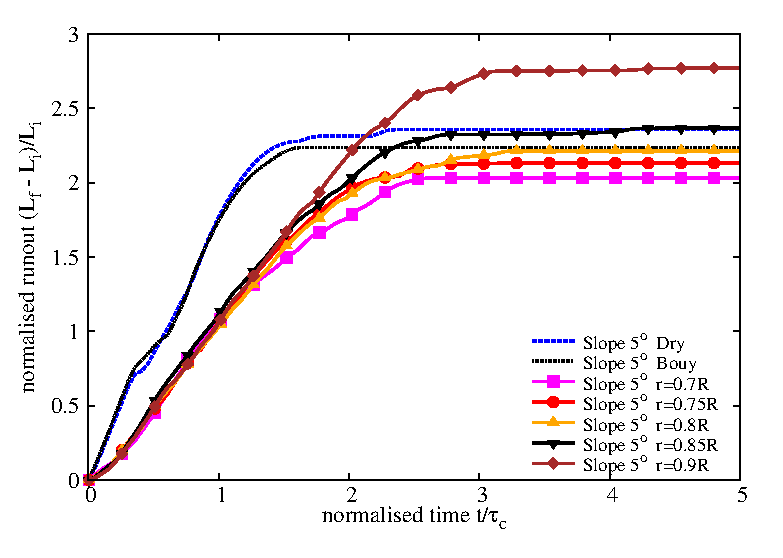
\includegraphics[width=0.97\columnwidth]{Runout_loose_5}
\caption{Evolution of run-out with time for different permeability (loose slope \SI{5}{\degree})}
\label{fig:run5}
\end{figure}


\begin{figure}
\centering
\includegraphics[width=0.97\columnwidth]{Height_loose_5}
\caption{Evolution of height with time for different permeability (loose slope \SI{5}{\degree})}
\label{fig:height5}
\end{figure}

\begin{figure}
\centering
\includegraphics[width=0.97\columnwidth]{KE_loose_5}
\caption{Evolution of Kinetic Energy with time for different permeability (loose slope \SI{5}{\degree})}
\label{fig:KE5}
\end{figure}

Positive pore-pressure generation at the base of the flow was observed for low 
permeable conditions. Inspection of the local packing density showed 
entrainment of water at the base of the flow, which can also be observed by the 
steep decrease in the packing density (see~\Cref{fig:voro5}) for the very low 
permeability condition (r = 0.9R). At the end of the flow ($t \ge 3 \times 
\tau_c$), the excess pore-pressure dissipates and the granular material, 
irrespective of their permeability, reaches almost the same packing density.

\begin{figure}
\centering
\includegraphics[width=0.97\columnwidth]{Voronoi_5}
\caption{Evolution of packing density with time for different permeability (loose slope \SI{5}{\degree})}
\label{fig:voro5}
\end{figure}

\subsection{Summary}

Two-dimensional LB-DEM simulations were performed to understand the behaviour 
of submarine granular flows. Unlike dry granular collapse, the run-out 
behaviour in fluid is dictated by the initial volume fraction. Granular columns 
with loose packing tend to flow longer in comparison to dense columns, due to 
entrainment of water at the base resulting in lubrication. The loose column 
when it starts flowing expands and ejects liquid, leading to a partial 
fluidization of the material. However, with increase in the slope angle, the 
run-out in fluid is influenced by the viscous drag on the granular materials. 
The run-out distance in fluid increases with decrease in permeability. More 
research work is required to characterise the flow behaviour of granular 
materials, especially in submerged conditions.
